\section{Two dimensions}
\todo{@TL: Stuff}
In 2-d we have 
\begin{equation}\label{eqn:Q1}
\cot \delta_{0}(p)-i=\frac{4}{m} \left(\frac{-1}{C_{0}(\Lambda)}+I_{0}(p, \Lambda)\right)\ ,
\end{equation}
and
\begin{equation}\label{eqn:Q2}
\cot\delta_0(p)=\frac{2}{\pi}\log(p a_0)\ ,
\end{equation}
where $a_0$ is the s-wave scattering length.  I assume a hard cutoff $\Lambda$, which can be most easily identified with the inverse lattice spacing of any numerical lattice calculation.  The term $I_0$ is
\begin{equation}\label{eqn:I0}
I_0(p,\Lambda)=\frac{1}{(2 \pi)^{2}} \int^{\Lambda} \mathrm{d}q_x\mathrm{d}q_y\ \left[\mathcal{P}\left(\frac{1}{\frac{p^2}{m}-\frac{\bm{q}^{2}}{m}}\right)-i \pi m\delta(\bm q^2-p^2)\right]\ .
\end{equation}

\subsection{Result in polar coordinates}
We first do the calculation in polar coordinates.  In this case eq.~\eqref{eqn:I0} becomes
\begin{align}
I_0(p,\Lambda)&=\frac{m}{(2 \pi)} \int^{\Lambda}_0 \mathrm{d}q \ q\ \left[\mathcal{P}\left(\frac{1}{p^2-q^{2}}\right)-i \pi \delta(q^2-p^2)\right]\\
&=\frac{m}{(2 \pi)} \int^{1}_0 \mathrm{d}\tilde q\  \tilde q\ \left[\mathcal{P}\left(\frac{1}{\tilde p^2-\tilde q^{2}}\right)-i \frac{\pi}{2|\tilde q|} \delta( \tilde q-\tilde p)\right]\\
&=\frac{m}{(2 \pi)} \int^{1}_0 \mathrm{d}\tilde q\ \mathcal{P}\left(\frac{\tilde q}{\tilde p^2-\tilde q^{2}}\right)-i \frac{m}{4}  \,\label{eqn:Q3}
\end{align}
where $\tilde q=q/\Lambda$ and $\tilde p=p/\Lambda$.  \texttt{Mathematica} tells me that this integral can be done,
\begin{align}
\frac{m}{(2 \pi)} \int^{1}_0 \mathrm{d}\tilde q\ \mathcal{P}\left(\frac{\tilde q}{\tilde p^2-\tilde q^{2}}\right)&=
\frac{m}{(2 \pi)} \log\left(\frac{\tilde p}{\sqrt{1-\tilde p^2}}\right)\\
&=\frac{m}{2 \pi} \log\left(\frac{p}{\Lambda}\right)+\frac{m}{4 \pi}\tilde p^2+\frac{m}{8 \pi}\tilde p^4+\mathcal{O}(\tilde p^6)\ ,
\end{align}
where in the second line I expanded in small $\tilde p$. Combining this result with eqs.~\eqref{eqn:Q1} and~\eqref{eqn:Q2} gives
\begin{align}
\frac{2}{\pi}\log(p a_0)&=\frac{4}{m} \left(\frac{-1}{C_{0}(\Lambda)}+\frac{m}{2 \pi} \log\left(\frac{p}{\Lambda}\right)+\mathcal{O}(\tilde p^2)\right)\nonumber\\
&=\frac{4}{m} \frac{-1}{C_{0}(\Lambda)}+\frac{2}{\pi}\log\left(\frac{p}{\Lambda}\right)+\mathcal{O}(\tilde p^2)\ ,
\end{align}
which implies that
\begin{equation}
 \frac{-1}{C_{0}(\Lambda)}=\frac{m}{2\pi}\log\left(a_0\Lambda\right)\ .
 \end{equation}

  
 \subsection{Result in cartesian coordinates}
We again start with eq.~\eqref{eqn:Q3} but express the integral in cartesian coordinates,
 \begin{equation}
 \frac{m}{(2 \pi)^2}4 \int^{1}_0 \mathrm{d}\tilde q_x\mathrm{d}\tilde q_y\ \mathcal{P}\left(\frac{1}{\tilde p^2-\tilde q_x^{2}-\tilde q_y^{2}}\right)-i \frac{m}{4} \ .
 \end{equation}
 The factor of 4 comes from using the symmetry of the kernal under $\tilde q_i\mapsto-\tilde q_i$, and therefore reducing the integration region
 \begin{displaymath}
 \int_{-1}^1d\tilde q_i\mapsto2\int_0^1d\tilde q_i\ .
 \end{displaymath}
 
The logarithmic divergence is present whether one does cartesian or polar integration.  The issue is the constant offset when doing the cartesian integration.  This offset comes from the corners of the integration of the Brillouin zone.  In 2-d, this offset is a finite number, and so we can just try to directly calculate the integral in these corners.  A little monkeying around shows that this offset is given by
\begin{equation}
\text{offset} = \left.8\int_0^{\pi/4}d\phi\int_1^{R(\phi)}dr\frac{r}{\tilde p^2-r^2}\right|_{\tilde p=0}\ .
\end{equation}
where $R(\phi)=1/\cos(\phi)$.  This expression represents the area of the box \emph{less} the contribution from the unit circle integration.  The factor of 8 is due to the fact that there are 8 or these regions that must be summed.  {\bf I should make a figure!}  Doing the first integral gives
\begin{equation}
-4\int_0^{\pi/4}d\phi \log\left(\frac{\tilde p^2-\cos(\phi)^{-2}}{\tilde p^2-1}\right)\ .
\end{equation}
Even though we cannot directly evaluate this integral, there is nothing pathologically wrong with it (i.e. no divergences).  We can do a series expansion of the kernal and integrate the expansion and get
\begin{equation}
4 \left(G-\frac{\pi}{2}\log(2)\right) - \frac{1}{2} \tilde p^2 (-2 + \pi) - 
 \frac{1}{16}\tilde p^4 (-8 + 5 \pi) +\mathcal{O}(\tilde p^6)\ .
\end{equation}
Setting $\tilde p=0$ gives us the offset.

\subsection{Determing $C_0(\Lambda)$}
Now that we have a stable counterterm, we can combine everything into the quantization condition (making sure I account for factors of $m$ and $\pi^2$, etc.) and get
\begin{align}
\frac{2}{\pi}\log(p a_0)&=\frac{4}{m} \left(\frac{-1}{C_{0}(\Lambda)}+\frac{m}{2 \pi} \log\left(\frac{p}{\Lambda}\right)+\frac{m}{\pi^2}\left(G-\frac{\pi}{2}\log(2)\right)+\mathcal{O}(\tilde p^2)\right)\nonumber\\
&=\frac{4}{m} \frac{-1}{C_{0}(\Lambda)}+\frac{2}{\pi}\log\left(\frac{p}{\Lambda}\right)+\frac{4}{\pi^2}\left(G-\frac{\pi}{2}\log(2)\right)+\mathcal{O}(\tilde p^2)\ .
\end{align}
For this equality to hold, we must have
\begin{equation}\label{eqn:ta da}
\boxed{
 \frac{-1}{C_{0}(\Lambda)}=\frac{m}{2\pi}\log\left(a_0\Lambda\right)-\frac{m}{\pi^2}\left(G-\frac{\pi}{2}\log(2)\right)
 }\ .
 \end{equation}
We display the coefficient to 15 decimal places,
\begin{displaymath}
G-\frac{\pi}{2}\log(2)=-0.1728274509745820501957409\ldots
\end{displaymath}

\section{Cartesian $S_2$}
We have
\begin{equation}
 \frac{-1}{C_{0}(\Lambda)}+\frac{1}{L^2}\sum_{q_i\in\ (-\Lambda,\Lambda]}\frac { 1 } { E - \frac{\bm{q}^2}{m} }=0\ .
 \end{equation}
 Using eq.~\eqref{eqn:ta da} gives
\begin{multline}
\frac{m}{2\pi}\log\left(a_0\Lambda\right)-\frac{m}{\pi^2}\left(G-\frac{\pi }{2}\log(2)\right)=-\frac{1}{L^2}\sum_{q_i\in\ (-\Lambda,\Lambda]} \frac { 1 } { E - \frac{\bm{q}^2}{m} }\\
\implies
\frac{2}{\pi}\log (pa_0)+\frac{2}{\pi}\log(\Lambda/p)=-\frac{4}{mL^2}\sum_{q_i\in\ (-\Lambda,\Lambda]}  \frac { 1 } { E - \frac{\bm{q}^2}{m} }+\frac{4}{\pi^2}\left(G-\frac{\pi}{2}\log(2)\right)\\
\implies
\frac{2}{\pi}\log (pa_0)=-\frac{4}{mL^2}\sum_{q_i\in\ (-\Lambda,\Lambda]}  \frac { 1 } { E - \frac{\bm{q}^2}{m} }-\frac{2}{\pi}\log(\Lambda/p)+\frac{4}{\pi^2}\left(G-\frac{\pi}{2}\log(2)\right)
\end{multline}
If we use the phase shift relation for 2-d, $\cot\delta(p)=\frac{2}{\pi}\log (pa_0)$ and replace $E=p^2/m$, then we have
\begin{align}
\cot\delta(p)&=-\frac{4}{mL^2}\sum_{q_i\in\ (-\Lambda,\Lambda]}  \frac { 1 } { \frac{p^2}{m} - \frac{\bm{q}^2}{m} }-\frac{2}{\pi}\log\left(\frac{\Lambda}{p}\right)+\frac{4}{\pi^2}\left(G-\frac{\pi }{2}\log(2)\right)\\
&=-\frac{4}{L^2}\sum_{q_i\in\ (-\Lambda,\Lambda]}  \frac { 1 } {p^2 - \bm{q}^2 }-\frac{2}{\pi}\log\left(\frac{\Lambda}{p}\right)+\frac{4}{\pi^2}\left(G-\frac{\pi }{2}\log(2)\right)\\
&=4\sum_{q_i\in\ (-\Lambda,\Lambda]}  \frac { 1 } {(\bm{q}L)^2-(pL)^2 }-\frac{2}{\pi}\log\left(\frac{\Lambda L}{pL}\right)+\frac{4}{\pi^2}\left(G-\frac{\pi }{2}\log(2)\right)\\
&=\frac{1}{\pi^2}\sum_{q_i\in\ (-\Lambda,\Lambda]}  \frac { 1 } {\left(\frac{\bm{q}L}{2\pi}\right)^2-\left(\frac{pL}{2\pi}\right)^2 }-\frac{2}{\pi}\log\left(\frac{\Lambda L}{pL}\right)+\frac{4}{\pi^2}\left(G-\frac{\pi }{2}\log(2)\right).
\end{align}
We now define the \emph{cartesian} $S_2$\label{eqn:S2}\footnote{For comparison, the \emph{spherical} (polar) $S_2$ function is
\begin{equation}\label{eqn:S2 polar}
S_2(x)\equiv\sum_{|\bm n|\le\Lambda'}\frac { 1 } { \bm{n}^2 -x}-2\pi\log\left(\Lambda'\right)\ .
\end{equation}}
\begin{align}
S_2(x)\equiv&\sum_{n_i\in\ (-\Lambda',\Lambda']}\frac { 1 } { \bm{n}^2 -x}-2\pi\log\left(\Lambda'\right)+4\left(G-\frac{\pi }{2}\log(2)\right)\\
=&\sum_{n_i\in\ (-\Lambda',\Lambda']}\frac { 1 } { \bm{n}^2 -x}-2\pi\log\left(\mathcal{L}_\square\Lambda'\right)\ ,
\end{align}
where $\Lambda'=\frac{\Lambda L}{2\pi} \in\ \mathbb{N}$ and
\begin{equation}
\mathcal{L}_\square=\exp\left(\log(2)-G\frac{2}{\pi}\right)=1.116306393581637659468497\ldots
\end{equation}
So we finally have
\begin{equation}\label{eqn:S2}
\cot\delta(p)=\frac{1}{\pi^2}S_2\left(\left(\frac{p L}{2\pi}\right)^2\right)+\frac{2}{\pi}\log\left(\frac{pL}{2\pi}\right)\ .
\end{equation}
Because of the logarithmic dependence in $p$ of the phase shift relation in 2-d, it is instead more convenient to move the logarithmic term on the RHS of the above equation to the LHS, which cancels the logarithmic dependence on $p$,
\begin{equation}
\frac{2}{\pi}\log\left(\frac{2\pi a_0 }{L}\right)=\frac{1}{\pi^2}S_2\left(\left(\frac{p L}{2\pi}\right)^2\right)\ .
\end{equation}

\subsection{Zero-range contact interaction}

\subsection{Finite-range interaction}
Here we use a separable potential of the form
\begin{equation}
V(\bm p',\bm p)=\frac{4}{m}\mathcal{C}f(\bm p')f(\bm p)\ .
\end{equation}
One can show that the discrete box eigenvalues $x=\frac{mL^2E}{4\pi^2}$ satisfy the self-consistency equation
\begin{equation}\label{eqn:SE}
\frac{1}{\mathcal{C}}+\frac{1}{\pi^2}\sum_{\bm n\in\mathrm{B.Z.}}\frac{f\left(\frac{2\pi}{L}\bm n\right)^2}{\bm n^2-x}=0\ .
\end{equation}
where $\bm n\in\mathrm{B.Z.}$ represents $\bm n\in(-N/2,N/2]^2$ and $N$ is the number of sites per side of the box.  Note that $\mathcal{C}$ is dimensionless in 2-d.  With a little math and manipulation, the phase shift can be determined with this separable interaction,
\begin{equation}\label{eqn:cot d}
\cot \delta(p) = \frac{1}{f(p)^2}\left(-\frac{1}{\mathcal{C}}+\frac{2}{\pi}\int_0^\infty dq \ \mathcal{P}\frac{qf(q)^2}{p^2-q^2}\right)\ .
\end{equation}

\subsubsection{Specific potentials}
Our first example uses the following separable potential,
\begin{equation}\label{eqn:potential1}
f(p)=\frac{1}{\sqrt{1+(p/\Lambda)^2}}\ .
\end{equation}
In this case one has
\begin{equation}
\frac{2}{\pi}\int_0^\infty dq \ \mathcal{P}\frac{qf(q)^2}{p^2-q^2}=\frac{2}{\pi}\int_0^\infty dq \ \mathcal{P}\frac{q}{(p^2-q^2)(1+(p/\Lambda)^2)}=\frac{2}{\pi}\frac{\log\left(\frac{p}{\Lambda}\right)}{1+(p/\Lambda)^2}\ .
\end{equation}
Equation~\eqref{eqn:cot d} becomes
\begin{equation}\label{eqn:first phase shift}
\cot\delta(p)=-\frac{1+(p/\Lambda)^2}{\mathcal{C}}+\frac{2}{\pi}\log\left(\frac{p}{\Lambda}\right)\ .
\end{equation}
Without loss of generality, we trade the dimensionless coefficient $\mathcal{C}$ with a dimensional (length) parameter $a_0$ via the relation
\begin{equation}
-\frac{1}{\mathcal{C}}=\frac{2}{\pi}\log(a_0\Lambda)\ .
\end{equation} 
Equation~\eqref{eqn:first phase shift} becomes
\begin{equation}
\cot\delta(p)=\frac{2}{\pi}\log(a_0p)+\frac{p^2}{2}\left[\frac{4\log(a_0\Lambda)}{\pi\Lambda^2}\right]\ .
\end{equation}

So we tested this potential and L\"uscher's formula is working.  Here we use the parameters
\begin{align*}
a_0&=2 \\
L&=10 \\
N&=100\\
\Lambda&= 5\\
\cot\delta(p)&=\frac{2}{\pi} \log (2 p)+0.0586348 \ p^2\ .
\end{align*}
With these parameters we determined the eigenenergies $x$ by numerically finding the roots of eq.~\eqref{eqn:SE} and then feeding these values through eq.~\eqref{eqn:S2}. The left panel of \autoref{fig:cotd1} shows these results.  The right panel uses $a_0=1$, which in this case supports negative $x$ solution.
\begin{figure}
\center
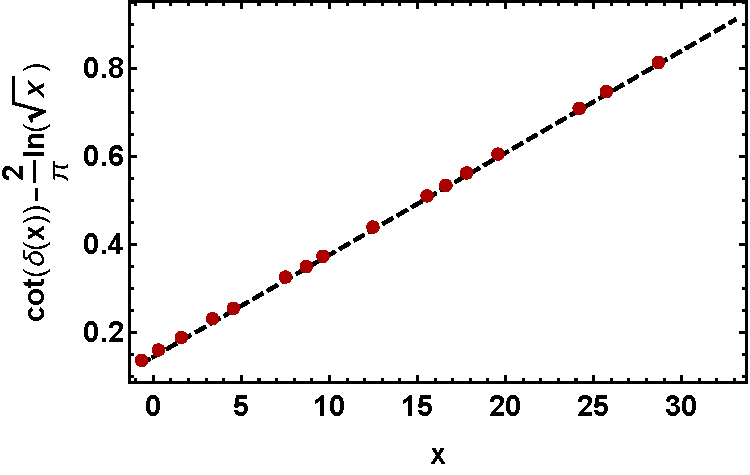
\includegraphics[width=.4925\textwidth]{figure/cotd1.pdf}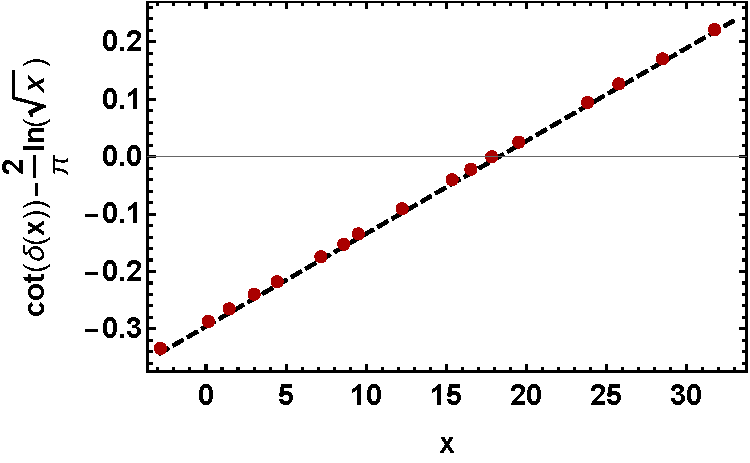
\includegraphics[width=.5075\textwidth]{figure/cotd4.pdf}
\caption{Dashed line is the exact result, the red dots are numerical results.  The potential in this case is given by eq.~\eqref{eqn:potential1}.  Left panel does not support a negative energy solution ($2\pi a_0/L>1$), right panel does ($2\pi a_0/L<1$).\label{fig:cotd1}}
\end{figure}
The agreement between L\"uscher and exact is pretty good.  We have confirmed that as I increase $N$, the points converge to the exact line.  

Our second example uses
\begin{equation}\label{eqn:potential2}
f(p)=\frac{1}{(1+(p/\Lambda)^2)^2}\ .
\end{equation}
Setting
\begin{equation}
\frac{-1}{\mathcal{C}}=\frac{2 \log (a \Lambda )}{\pi }-\frac{11}{6 \pi }\ ,
\end{equation}
we find 
\begin{equation}
\cot \delta(p)=\frac{2 \log (a p)}{\pi }+\frac{p^2 (24 \log (a \Lambda )-13)}{3 \pi  \Lambda ^2}+\frac{p^4 (24 \log (a \Lambda )-19)}{2 \pi  \Lambda
   ^4}
  +\frac{p^6 (8 \log (a \Lambda
   )-7)}{\pi  \Lambda ^6} -\frac{p^8 (11-12 \log (a \Lambda ))}{6 \pi  \Lambda ^8}\ .
\end{equation}
Using the following parameters,
\begin{align*}
a_0&=2 \\
L&=10 \\
N&=100\\
\Lambda&= 5\ ,
\end{align*}
We find good agreement between L\"uscher and the exact result, as shown in the left panel of~\autoref{fig:cotd23}.
\begin{figure}
\center
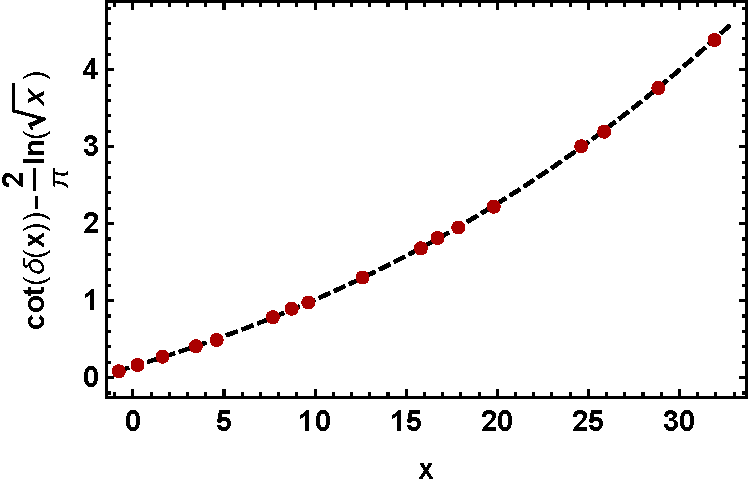
\includegraphics[width=.485\textwidth]{figure/cotd2.pdf}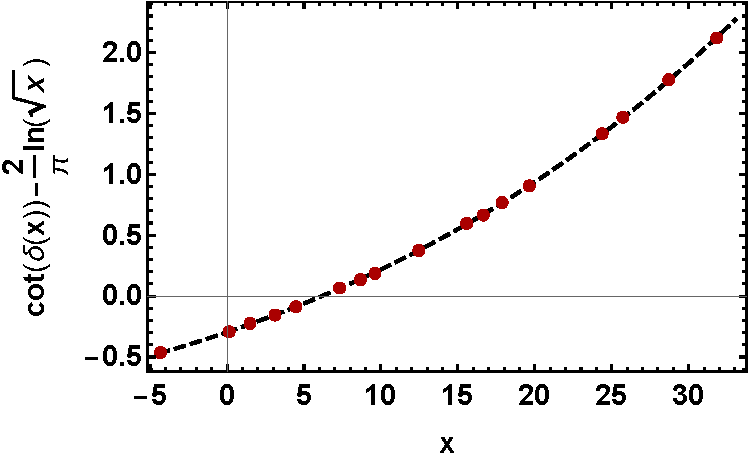
\includegraphics[width=.515\textwidth]{figure/cotd3.pdf}
\caption{Dashed line is the exact result, the red dots are numerical results.  The potential in this case is given by eq.~\eqref{eqn:potential2}.  Left panel does not support a negative energy solution ($2\pi a_0/L>1$), right panel does ($2\pi a_0/L<1$).\label{fig:cotd23}}
\end{figure}
We also reduce the scattering length such that it supports a negative energy solution, $a_0=1$.  The right panel of~\autoref{fig:cotd23} shows this case.  Again, there is good agreement between exact and L\"uscher.